% !TeX root = ../complete.tex
\section{قطع تغذیه بلوک با \lr{Power Gating}}
\label{sec:power-gating}

\subsection{مسیر تغذیه، جداسازی خروجی و حفظ وضعیت}
\label{sec:power-gating-operation}

در \NotesTopic{sec:power-clock-gating}{\lr{Clock Gating}}، ساعت
بلوک متوقف می‌شود و ریل تغذیه به مدار وصل می‌ماند. در \lr{Power Gating}،
یک ترانزیستور سری، مسیر تغذیه بلوک را در حالت خواب قطع می‌کند.
در شکل \ref{fig:power-gating-header}، یک \lr{pMOS Header} میان
تغذیه اصلی \(V_{DD}\) و ریل تغذیه بلوک قرار دارد. ولتاژ ریل بعد
از کلید را \(V_{DDV}\) می‌نامیم. آن را ریل تغذیه مجازی می‌گویند،
زیرا مقدارش به وضعیت کلید، بار و نشتی بلوک وابسته است. گزینه‌ی دیگر
\lr{nMOS Footer} است که به‌جای تغذیه بالا، مسیر اتصال به زمین را
قطع می‌کند \cite[بخش \secnum{۵.۳.۲}، صفحات ۱۹۷ و ۱۹۸]{weste}
\cite[اسلاید ۲۳]{powerslides}.

\begin{figure}[htbp]
  \centering
  \begin{latin}
  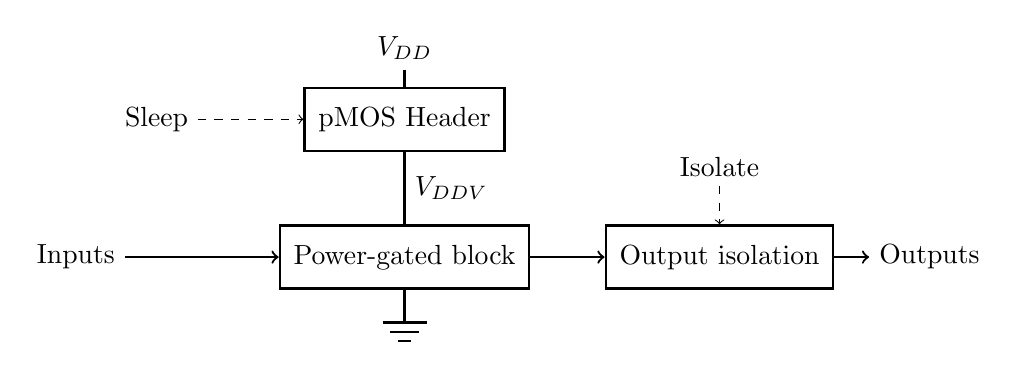
\begin{tikzpicture}[
    x=1cm,y=1cm,
    component/.style={draw,thick,minimum height=8mm,align=center,inner sep=5pt}
  ]
    \node[component] (header) at (0,1.75) {pMOS Header};
    \node[component] (block) at (0,0) {Power-gated block};
    \node[component] (isolate) at (4,0) {Output isolation};
    \node (supply) at (0,2.65) {\(V_{DD}\)};
    \node (sleep) at (-3.15,1.75) {Sleep};
    \node (clamp) at (4,1.15) {Isolate};
    \draw[thick] (supply) -- (header.north);
    \draw[thick] (header.south) -- (block.north)
      node[midway,right] {\(V_{DDV}\)};
    \draw[dashed,->] (sleep.east) -- (header.west);
    \draw[dashed,->] (clamp.south) -- (isolate.north);
    \draw[->,thick] (-3.55,0) node[left] {Inputs} -- (block.west);
    \draw[->,thick] (block.east) -- (isolate.west);
    \draw[->,thick] (isolate.east) -- (5.9,0) node[right] {Outputs};
    \draw[thick] (block.south) -- (0,-0.83);
    \draw[thick] (-0.28,-0.83) -- (0.28,-0.83);
    \draw[thick] (-0.18,-0.95) -- (0.18,-0.95);
    \draw[thick] (-0.08,-1.07) -- (0.08,-1.07);
  \end{tikzpicture}
  \end{latin}
  \caption{مسیر تغذیه و مسیر داده در یک بلوک دارای \lr{Power Gating}.
    \lr{Sleep} کلید تغذیه را کنترل می‌کند و \lr{Isolate} سطح خروجی را
    هنگام قطع تغذیه معتبر نگه می‌دارد. طرح مفهومی از شکل \secnum{۵.۲۴}
    کتاب و اسلاید ۲۳ اقتباس شده است \cite{weste,powerslides}.}
  \label{fig:power-gating-header}
\end{figure}

در حالت فعال، کلید روشن است و ریل مجازی نزدیک \(V_{DD}\) می‌ماند.
در خواب، کلید خاموش می‌شود و بار ذخیره‌شده روی ریل مجازی می‌تواند
از مسیرهای نشتی کاهش یابد. تا زمانی که تغذیه بلوک دوباره برقرار شود،
خروجی آن ممکن است در محدوده نامعتبر بین صفر و یک بماند. مدار
\lr{Output Isolation} با تغذیه برقرار، پیش از قطع تغذیه خروجی را
به یک سطح مشخص مانند صفر محدود می‌کند. اگر بلوک باید پس از بیداری
از همان داده ادامه دهد، داده را در \lr{Retention Register} با تغذیه
برقرار یا در حافظه‌ای بیرون از دامنه‌ی خاموش نگه می‌دارند. پس از
وصل تغذیه، ریل فرصت بازیابی دارد و وضعیت لازم بازیابی یا مقداردهی
اولیه می‌شود. جداسازی هنگامی برداشته می‌شود که خروجی‌های بلوک معتبر
باشند \cite[بخش \secnum{۵.۳.۲}، صفحات ۱۹۷ تا ۱۹۹]{weste}.

\subsection{افت روی کلید و اثر آن بر تأخیر}
\label{sec:power-header-delay}

در یک برآورد دست‌اول برای کلید روشن، \(W\) عرض مؤثر کلید،
\(R_h\) مقاومت روشن و \(r_w\) حاصل‌ضرب مقاومت روشن در عرض است.
\(r_w\) برای طول کانال و شرایط بایاس مشخص داده می‌شود و می‌توان آن
را با اهم‌میکرومتر بیان کرد. اگر جریان نماینده‌ی بلوک در حالت فعال
\(I_{\mathrm{on}}\) باشد، قانون اهم افت ریل را به عرض کلید ربط می‌دهد.
\begin{equation}
  R_h\approx\frac{r_w}{W},\qquad
  \Delta V=V_{DD}-V_{DDV}\approx I_{\mathrm{on}}R_h.
  \label{eq:power-header-droop}
\end{equation}
ضرب آمپر در اهم واحد ولت دارد. بزرگ‌تر کردن عرض، در این مدل
مقاومت و افت را کاهش می‌دهد. به‌کارگیری جریان متوسط برای بلوک بزرگ
هنگامی مناسب‌تر است که رویدادهای سوئیچینگ در زمان پخش شوند و ظرفیت
روی ریل مجازی، نوسان ولتاژ را هموار کند. اگر چند بار هم‌زمان جریان
زیادی بکشند، افت گذرا می‌تواند با برآورد متوسط تفاوت داشته باشد
\cite[بخش \secnum{۵.۳.۲.۱}، صفحات ۱۹۸ و ۱۹۹]{weste}.

برای مرتبط کردن افت ریل با تأخیر، \(V\) را ولتاژ مؤثر تغذیه بلوک،
\(V_t>0\) را آستانه‌ی مؤثر و \(D(V)\) را تأخیر مسیر در آن ولتاژ
می‌گیریم. برآورد فصل ۳ از تقسیم بار جابه‌جاشده بر جریان شروع می‌شود.
برای تغییر ولتاژ به اندازه‌ی کسری ثابت از \(V\)، بار با \(V\) متناسب
است. در \lr{Alpha-Power Law} جریان راه‌اندازی با \((V-V_t)^m\)
متناسب است. توان تجربی \(m\) معمولاً بین ۱ و ۲ است. کتاب آن را
\(\alpha\) می‌نویسد. در این فصل، \(\alpha\) برای \lr{Activity Factor}
به کار می‌رود. اگر ظرفیت و پارامترهای مدل ثابت باشند، برای \(V>V_t\)
با ثابت مثبت \(K\) داریم
\cite[رابطه \secnum{۴.۲۹}، صفحه ۱۶۲]{weste}.
\begin{equation}
  D(V)=K\frac{V}{(V-V_t)^m}.
  \label{eq:power-above-threshold-delay}
\end{equation}
\(K\) ظرفیت، ضرایب جریان و عوامل ثابت مربوط به مسیر را در بر می‌گیرد.
در این نوشتار، واحد آن \(\mathrm{s}\,\mathrm{V}^{m-1}\) است تا پس
از ضرب در \(V/(V-V_t)^m\)، حاصل واحد زمان داشته باشد. با تقسیم تأخیر ریل
مجازی بر تأخیر اولیه، \(K\) حذف می‌شود و نسبت زیر از مدل به دست می‌آید.
\begin{equation}
  \frac{D(V_{DD}-\Delta V)}{D(V_{DD})}
    =\left(1-\frac{\Delta V}{V_{DD}}\right)
      \left(\frac{V_{DD}-V_t}{V_{DD}-V_t-\Delta V}\right)^m.
  \label{eq:power-droop-delay-ratio}
\end{equation}
این نسبت برای \(0\leq\Delta V<V_{DD}-V_t\) تعریف شده است. اگر
افت صفر باشد، نسبت یک است. برای افت مثبت، عامل نخست کم‌تر از یک
و عامل دوم بزرگ‌تر از یک است. در این مدل با \(m\geq 1\)، کاهش
توانایی جریان‌دهی بر کاهش بار لازم برای گذار غلبه می‌کند.

برای افت کوچک می‌توان از حساسیت تأخیر استفاده کرد. اگر مقدار ولتاژ
از \(V\) به \(V-\Delta V\) برود، تقریب خطیِ تابع نزدیک \(V\)
می‌دهد \(D(V-\Delta V)-D(V)\approx-D'(V)\Delta V\).
برای محاسبه مشتق، \(D(V)=KV(V-V_t)^{-m}\) را به‌شکل ضرب دو
تابع می‌نویسیم. مشتق عامل اول \(K\) است. برای مشتق عامل دوم، قاعده
توان، \(-m(V-V_t)^{-m-1}\) را می‌دهد و طبق قاعده زنجیره‌ای آن را
در مشتق \(V-V_t\)، یعنی یک، ضرب می‌کنیم. حاصلِ قاعده ضرب پس از تقسیم بر
\(D(V)\)، دو جمله برای حساسیت باقی می‌گذارد. با \(V=V_{DD}\)
و \(\Delta D=D(V_{DD}-\Delta V)-D(V_{DD})\)، نتیجه چنین است.
\begin{equation}
  \frac{\Delta D}{D(V_{DD})}
  \approx\left(\frac{m}{V_{DD}-V_t}-\frac{1}{V_{DD}}\right)\Delta V.
  \label{eq:power-droop-delay-sensitivity}
\end{equation}
عبارت داخل پرانتز واحد معکوس ولت دارد و حاصل بی‌بعد است. هرچه
\(V_{DD}-V_t\) کوچک‌تر باشد، افت معین می‌تواند اثر نسبی بیشتری
بر تأخیر بگذارد. برای نمونه، با \(V_t/V_{DD}=0.30\) و \(m=1.4\)
عبارت داخل پرانتز \(1/V_{DD}\) است و در تقریب خطی درصد افزایش
تأخیر با درصد افت تغذیه برابر می‌شود. برابری درصدها به پارامترها
و کوچک بودن افت وابسته است.

\subsection{اندازه کلید و حداقل زمان خواب}
\label{sec:power-header-sizing}

اگر حد مجاز افت ریل \(\Delta V_{\max}>0\) معلوم باشد، با جای‌گذاری
\(R_h\) در رابطه \eqref{eq:power-header-droop} و اعمال شرط
\(\Delta V\leq\Delta V_{\max}\)، از مدل مقاومتی حد زیر بر عرض
به دست می‌آید. همه‌ی کمیت‌ها مثبت‌اند و ضرب و تقسیم جهت نامساوی
را تغییر نمی‌دهد.
\begin{equation}
  W\geq\frac{I_{\mathrm{on}}r_w}{\Delta V_{\max}}.
  \label{eq:power-header-width}
\end{equation}
در مثال ۵.۵ کتاب، تغذیه \qty{1}{\volt} و توان فعال میانگین حافظه
\qty{2}{\watt} است. تقسیم توان بر ولتاژ، جریان \qty{2}{\ampere}
را می‌دهد. کتاب برای بررسی افزایش تأخیرِ ۵ درصدی در همان مثال،
افت ریل را تقریباً ۵ درصدِ تغذیه می‌گیرد، یعنی
\qty{50}{\milli\volt}. مقاومت کلید از تقسیم این افت بر جریان
به‌دست می‌آید و حداکثر \qty{25}{\milli\ohm} است. برای
\(r_w=\qty{2}{\kilo\ohm\micro\metre}\) حد عرض چنین می‌شود
\cite[مثال ۵.۵، صفحات ۱۹۸ و ۱۹۹]{weste}.
\[
  W\geq\frac{\qty{2e3}{\ohm\micro\metre}}{\qty{25e-3}{\ohm}}
    =\qty{8e4}{\micro\metre}.
\]
واحد اهم ساده می‌شود و این عرض، مجموع عرض مؤثر کلیدهایی است که
می‌توان موازی بست. کتاب برای همان مثال از شبیه‌سازی مدار عرض کم‌تری
به دست می‌آورد و تفاوت را با تغییر مقاومت روشن در بایاس واقعی توضیح
می‌دهد. هنگام روشن شدن کلید، شارژ ریل مجازی می‌تواند جریان آغازین
بزرگی ایجاد کند. روشن کردن گروه‌های موازی در چند گام، روشی برای
محدود کردن این جریان آغازین است \cite[صفحه ۱۹۹]{weste}.

برای سنجش صرفه‌ی خواب، \(P_{\mathrm{idle}}\) را توان بلوک در حالت
بی‌کارِ دارای تغذیه، \(P_{\mathrm{sleep}}\) را توان بلوک در خواب و
\(E_{\mathrm{tr}}\) را انرژی اضافیِ ورود و خروج از خواب بگیرید.
اگر \(P_{\mathrm{idle}}>P_{\mathrm{sleep}}\)، در مدت خواب \(T_s\)
به‌اندازه‌ی \((P_{\mathrm{idle}}-P_{\mathrm{sleep}})T_s\) انرژی
صرفه‌جویی می‌شود. خواب هنگامی از لحاظ انرژی به‌صرفه است که این مقدار
از \(E_{\mathrm{tr}}\) بیشتر باشد. با حل نامساوی برای زمان، شرط
به صورت زیر است \cite[بخش \secnum{۵.۳.۲}، صفحات ۱۹۷ و ۱۹۸]{weste}.
\begin{equation}
  T_s > T_{\mathrm{BE}}
      =\frac{E_{\mathrm{tr}}}{P_{\mathrm{idle}}-P_{\mathrm{sleep}}}.
  \label{eq:power-gating-break-even}
\end{equation}
\(T_{\mathrm{BE}}\) زمان سربه‌سر انرژی است. ژول تقسیم بر وات
ثانیه می‌دهد. برای نمونه، اگر هزینه تغییر حالت \qty{1}{\nano\joule}
و کاهش توان \qty{2}{\milli\watt} باشد، تقسیم
\qty{1e-9}{\joule} بر \qty{2e-3}{\watt} برابر
\qty{0.5}{\micro\second} است. جدا از صرفه‌ی انرژی، زمان بیداری
نیز باید با مهلت پاسخ سامانه سازگار باشد.
